\documentclass[14pt]{article}
\usepackage[utf8]{inputenc}
\usepackage{xcolor}
\usepackage{hyperref}
\usepackage{graphicx}
% \usepackage{wrapfig}
\usepackage{amsmath}
\usepackage{algorithm}
\usepackage{algorithmic}
\usepackage{array}
\hypersetup{
    colorlinks=true,
    linkcolor=blue,
    filecolor=magenta,      
    urlcolor=cyan,
    pdftitle={Overleaf Example},
    pdfpagemode=FullScreen,
    }
    
%\usepackage[left=1.00cm, right=1.00cm, top=0.75cm, bottom=1.25cm]{geometry} 
% \usepackage[left=0.30cm, right=5.70cm, bottom=1.55cm, top=0.75cm]{geometry}
\usepackage[left=2.15cm, right=2.15cm, bottom=1.55cm, top=0.75cm]{geometry}

\newcommand{\remark}[1]{{\color{purple} (#1)}}

\title{\sc{Lakat}\break \sc{A Publishing Architecture}}
\author{Leonhard Horstmeyer \\
\remark{Do not distribute}}
\date{\today}

\begin{document}


\maketitle

\tableofcontents

\begin{abstract}
    
\end{abstract}
\section{Introduction}

With the vast spectrum of data structures, of query and storage systems, of versioning and networking tools, one may create publishing systems that satisfy certain desirables, rather than incrementally adjusting the existing one. Starting from a set of requirements for such a system we propose one architecture around the available technology that we call \textit{Lakat}, whilst acknowledging and demarcating it from other proposals. We discuss typical user journeys and attack vectors.

We start with a set of eight core requirements, that we posit for a publishing system. It should be open, permissionless, pluralistic, process-oriented, curatable and sustainable. It should make conflict resolution manifest and allow for AI to participate and contribute. We will discuss these requirements in detail in the next section. We propose a distributed database with a local peer-reviewed concensus layer. The system serves as a continuous integration and continuous development (CI/CD) solution for collaborative research and one may conceptionally think of Lakat as a decentralized version of wikipedia with a branch structure similar to git and a peer review system on top.

The entire architecture of Lakat is heavily inspired by concepts developed by the Hungarian philosopher Imre Lakatos. Probably in an attempt to contribute to the demarcation problem that was prominent in the field of philosophy of science during Lakatos' times and still these days, he developed the concept of a \textit{research programme}, which is also called \textit{Lakatosian research programme} to avoid confusion with the colloquial use of the former term. The demarcation problem asks what it is that sets science apart from pseudo-science. Steering clear of a circular definition of pseudo-science throught the demarcation this problem simply asks "What is science"? We refer the interested reader to the pertinent literature and go on to mention that Lakatos develops his theory on the grounds of a process-oriented account of science. So rather than saying that this or that monolitic bulk of work or set of statements is science or not, he posits that it only processes of amendments to a corpus of previous amendments can be indicative of being science or not. To that end he distinguishes progressive and degenerative amendments. For Lakatos a research programme consists of a \textit{hard core}, which is a set of constituting assumptions, axioms as it were, that capture the essence of a research endeavor and a \textit{protective belt} of auxiliary hypothesis. The assumptions in a core are constituting in the sense that the research programme would cease to exist without them. Rather than saying -- as one might imagine -- that the science--predicate of research programmes relies on modifications of this hard core, he instead endows them with dogmatic immutability, disallowing any hypothetical modifications of them. In a quest for guarding this sacred hard core a research programme can only make amendments to the protective belt that ought to divert possible attacks to the core. An attack cosists in a conflict of the theory with empiric evidence. 


which in lakat correspond to proper branches. For him additions to the research programme can render it progressive or degenerative, which is where he ultimately draws the line between science and pseudoscience. 

Which problems does it solve?

Comparison to other solutions. 
``DeSci Labs'', ``Lateral.io'', ``Publishing DAO'', ...

\section{Requirements}

In this section we provide a list of high-level requirements that we wish to be satisfied by a publication system. We then consider three existing publishing systems in view of those requirements:

\indent \textbf{1. Open} -- 
 Content and code base\footnote{Here we refer to the code base of any client implementation.} should be accessible freely\footnote{Internet service providers are not free. So we refer here to additional charges.}.\\
\indent\textbf{2. Permissionless} --
 No one should be barred from contributing.\\
\indent\textbf{3. Pluralistic} -- No monopoly on research opinion.\footnote{This is not not necessarily the same as ``No single source of truth''.}\\
\indent\textbf{4. Process-oriented} -- Putting the curation on par with the content.\\
\indent\textbf{5. Conflict-oriented} -- Making irreconcilabilities manifest.\\
\indent\textbf{6. Curatable} -- Putting the curation on par with the content.\\
\indent\textbf{7. Sustainable} -- 
 Data and compute resources should be low and reuse of fragments encouraged.\\
%  \item \textbf{soft constraints}
\indent\textbf{8. AI friendly} -- AI should be able to interact with the system.\\

The classical route to publishing is through sending a manuscript to the editors of a peer reviewed journal. The editor(s) then search(es) for reviewers willing to review the manuscript. Is this open? In most cases the article as well as the review, the code base and the data -- if there is any --  are locked behind pay walls, i.e. not accessible publicly. Some journals have various open access options, that allow the abovementioned parts of the publication to be accessible, albeit at a high price for the author both in terms of money and in terms of transferral of rights to the publisher. In principle the system is permissionless, except for those cases where publication fees apply and/or membership in a recognised institution is required. This system is not particularly monopolous, at least prima facie. The de facto sovereignty over what is an exceptable contribution rests with the editor(s) of the journals, but given enough funding new journals can form. The process of the research as well as the review are not well mapped in this system. There is no focus and in particular no build-in focus on resolution of conflicting results. Curation is left to the editors. 

Wikipedia\footnote{Here we refer not only to the software implementation, which at the time of writing is version 1.39 of mediawiki, publicly accessible via wikipedia.org (April 2023), but also the body of editors and maintainers.} is an open database. Both its code-base as well as its content can be viewed with access to a non-censored internet connection. A large part of the database can be edited permissionlessly, even without an account. Every article has one current version, often with a rich history of older versions and vivid discussions around edits. At times fierce editing battles can be observed and have been subjected to scientific studies \cite{dedeo}. 
The possibility to express different views on a matter in the form of versions as well as the discussion adds a pluralistic element, even though the existence of a single current truth in the form of the latest version of an article deducts from that. the multilingual featuer on the other hand makes wikipedia more pluralistic. 

Programmable blockchain is an open database. Is is often referred to as bein permissionless and that is true for most blockchains in the sense that no third party controls read or write access to it.


 Making a manifestly pluralist system not only prevents the dictatorship of one academic credo over another, but also allows for conflicting opinions to develope and hopefully to resolve.
 

\section{Elements of the Publishing System}

We propose a manifestly pluralistic, process and conflict-oriented architecture for the continuous integration and continuous development (CI/CD) of publications with a primary use case of research publications. At its core the architecture consists of a linked data structure that resembles a DAG, where the key objects are branches. This data structure facilitates collaborative work in much the same way as git does. Branches may be thought of as the analogue of a journal in traditional publishing (c.f. Subsection ???). The role of journal editors is covered largely by branch contributors. Branches are chains of blocks that contain submissions. Addition of another block happens via a proof of peer review, where the peers are the contributors to that branch. In that sense branches resemble block chains with blocks consisting of changes instead of transactions and the consensus is provided by a  proof of review, a local (i.e. involving just branch-contributors) consensus rather than a global one.
The review process follows a weak\footnote{Weak is to be understood in the sense that both parties may choose to reveal their identity.} form of a double-blind protocol, leveraging zero-knowlege proofs.
Data is content-addressable and conforms to the ipld format. Storage may be delegated to a selection of storage providers, including decentralized storage networks such as ipfs, storj and others to improve resiliance and longevity. In the following we discuss the individual elements of the proposed system and highlight their interaction.

\subsection{Data Structure}
\subsubsection{Bucket}
\label{ssc:bucket}
The most elementary data object is the \textit{bucket}. Each and every submitted item is submitted in a bucket: datasets, paragraphs, images and formulae are contained in buckets. These are examples of \textit{atomic buckets}, expressing the fact that they are the building blocks of the system. 
% We decisively opted against objects that represent traditional folders, where every file belongs to one and only one folder\footnote{In git the folder object is called a \textit{tree node} and it is not possible for a file (called a \textit{blob} in git-speak) to belong to multiple trees. In the unix filesystem it is only possible through the hack of soft and hard links.}.
Instead of a folder structure we solve the containment relation through designated buckets that we call \textit{molecular buckets}. The data part of those buckets contains merely an arrangement of atomic buckets. One may think of them as the analogue of an article, a book or some other curated content. 


\begin{figure}[h!]
  \begin{center}
    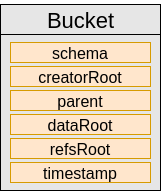
\includegraphics[width=0.20\textwidth]{img/DataBucketV2.png}
\end{center}
 \caption{The most elementary type of data container is the bucket. It contains only immutable entries (orange), such as the \textit{schema}, the \textit{creatorRoot}, the \textit{parent}, the \textit{dataRoot}, the \textit{refsRoot} and the \textit{timestamp}.}
 \label{fig:bucket}
\end{figure}


Every bucket contains six entries: A \textit{schema}, a \textit{creatorRoot}, a \textit{parent}, a \textit{dataRoot}, a \textit{refsRoot} and a \textit{timestamp}. See Figure \ref{fig:bucket} for an illustration. Here and henceforth the word root refers to the root of a Merkle tree. We go through the entries in turn. The \textit{schema} contains information about the format of the data. For instance we have already mentioned that the data in the molecular buckets is formatted as an arrangement\footnote{The purposefully vague formulation of an 'arrangement' is due to the intention to keep that format flexible. One may think of this as an ordered list, but one might also consider further directives or clustering of content in a directed hypergraph.}. The \textit{creatorRoot} points to information about the creator of this bucket. Identity on \textit{Lakat} is solved through proofs (see Section \ref{ssc:proofs}). The \textit{parent} is the \textit{content identifier} of the parent bucket. For genesis buckets that would be 0. The \textit{dataRoot} is a content identifier of the data contained in the bucket. In future versions the schema could be absorbed into the dataRoot using the ipld multihash format. This would require a Lakat-specific codec. The \textit{refsRoot} points to all the references made to other buckets within the data. This is necessary, since references to other buckets might be obscured inside the data-encoding. This is an analogue of a list of citations. The \textit{timestamp} records the time of inclusion of the bucket into the branch. It is important to note that we use ethereum block hashes as time stamps in our first version, since the local consensus is too weak to ensure that all participants are truthful to the time otherwise. Anticipating block hash is close to impossible. One cannot change the data inside the bucket. One would have to create a new bucket that points to the original bucket via its parent entry. 

\subsubsection{Branch}
\label{ssc:branch}

\begin{figure}[t!]
\begin{center}
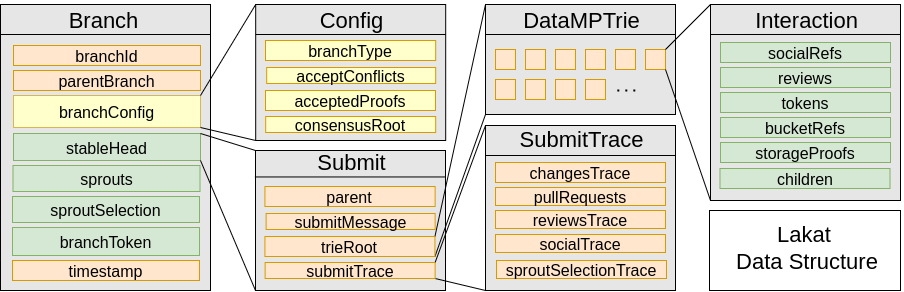
\includegraphics[width=\textwidth]{img/BranchV9.png}
\end{center}
 \caption{A schematic illustration of the branch object and its entries.}
 \label{fig:branchstructure}
\end{figure}
The central object type of Lakat is the \textit{branch}. See Figure \ref{fig:branchstructure} for an illustration. Branches represent journals or research communities. They share some properties with \textit{git}-branches and some with blockchains. Every branch contains an id, called \textit{branchID}, that uniquely identifies it. The immutable entries of a branch and the initial head are hashed to produce the branch identifier. The branch also points to a parent branch from which it was branched off. The corresponding entry is called \textit{parentBranch}. This construction turns the set of branches into a linked data structure.\footnote{\remark{Maybe check this} In \textit{git} a branch is simply pointer to the head commit. In blockchains one often encounters ids attached to the chain (so-called \textit{chainid}) to avoid issues when the consensus mechanism yields two differnt chains.} At creation time the branch receives a \textit{timestamp}. The previous entries are all immutable. There are then four mutable entries, namely \textit{stableHead}, then the two consensus entries \textit{sprouts} and \textit{sproutSelection} and finally \textit{branchToken}. The stable head is a pointer to the latest stable submit. A \textit{submit} is a set of changes (see Subsection \ref{ssc:submit} on submits). One may think of it as the Lakat version of an article submission. It has similiarities to a commit in git -- not only phonetically -- but also to a block in \textit{ethereum}. The addition of new submits works through a consensus mechanism called \textit{proof of review (PoR)} and \textit{lignification} (see Subsection \ref{ssc:consensus}). Also in this respect the branch behaves a lot like a blockchain. Every branch has it's own token, the \textit{branchToken}. It allows funding bodies to fund a particular branch. Token logic is not handled by \textit{Lakat}. Instead this entry essentially points to proofs of transactions on a blockchain where the respective token lives. The purpose of the integration of tokens is to create an incentive layer on top of Lakat, because (unfortunately) \textit{humans} as well as \textit{AI} do not work without incentives. The branch also carries configurational metadata, stored in \textit{branchConfig}. It points to information about the branch type, whether merge conflicts are accepted, the consensus rules and the proofs that are accepted, such as proofs of token transfer or proofs of time. The branchConfig's mutability is more constrained than that of the stable head (See Subsection \ref{ssc:configupdate}).


There are three types of branches: \textit{proper branches}, \textit{sprouts} and \textit{twigs}. The branch type is stored in the branch config and can be changed under certain conditions. 
\textit{Proper branches} can only be modified through the local consensus mechanism (see Subsection \ref{ssc:consensus}). They point to a non-empty set of sprouts, which help with the process of producing stable heads in the proper branch. Proper branches cannot be changed to any other branch type. A \textit{sprout} is a short-lived branch that is exclusively used to grow proper branches. Sprouts behave a bit like ommers in the ethereum protocol in the sense that they are contestors to produce the next stable head. Sprout branches point to an empty set of sprouts themselves. The sproutSelection contains all the sprouts that are rooted in it. The branchToken entries is empty. The stableHead is immutable. There is only one way to modify the sprout, namely indirectly when it turns into a proper branch during the lignification process (See Subsection \ref{ssc:lignification}). Finally, a \textit{twig} can be thought of a little feature branch. Twigs can be modified through submits by \textit{contributors} of the twig (See Subsection \ref{ssc:contributors} for more information on contributors) or through merges. However, the process of merging into a twig does not need to go through the consensus mechanism of proper branches (See Subsection \ref{ssc:consensus}).

In this paragraph we merely introduce some nomenclature. We distinguish between \textit{core} and \textit{belt} branches, which correspond to \textit{this} and \textit{other} in git. These are not intrinsic properties of branches, but denote the role they play during a merge. Lakat only has one type of merge. The core branch will be updated and the belt branch not (see Susbsection \ref{ssc:merge} for information on merges). A branch may be a core with respect to one merge and a belt with respect to another merge. This terminology originates in the core-belt dichotomy of Lakatosian research programmes. There is a further distinction that is purely conceptual and is not manifested in the technical specification, but in the nomenclature. We distinguish a \textit{derived branch} from a \textit{seedling branch} in that the seedling branch has a \textit{singularity submit} without a parent (See Subsection \ref{ssc:submit} for information on submits). A singularity submit corresponds to the genesis block in a blockchain. We invoke here a cosmological metaphore rather than a biblical one. The seedling branch has no parent branch and the corresponding entry points to zero. A derived branch on the other hand has a parent branch that it points to. We say that the derived branch is \textit{rooted} in the parent branch. The \textit{root} of a derived branch is the last submit in the submit history that is also in the history of the parent branch.

We also not that there are various levels at which Lakat can be viewed as a graph, going from high level to low level. At the level of the branches one can form a graph $\mathcal B$, where a branch is a node and a directed link from one branch $A$ to another branch $B$ means that $B$ is the parent of $A$ or that $B$ is merged into $A$ (See Subsection \ref{ssc:merge} regarding merging). This directed graph is not necessarily a-cyclic, because $A$ can be rooted in $B$ and merge back into $B$, however if one excludes merges it is. At the level of the submits, a graph $\mathcal S$ can be created with the submits being nodes and a link can be drawn from a submit $q$ to $p$ when $p$ is the parent of $q$. This yields a directed acyclic graph (DAG). Finally at the level of the data buckets there exists a graph structure $\mathcal D$ induced by the parent reference inside the bucket. There is a graph homomorphism from $\mathcal S$ to $\mathcal B$, but not vice versa and there are no homomorphisms between $\mathcal S$ and $\mathcal D$ or $\mathcal B$ and $\mathcal D$. The lack of a homomorphism between the submit structure and the data structure indicates that these are two separate layers. The relation between the elementary bucket object and the higher level branch object is not simply a many-to-one relation. Different branches may share the some data buckets. In practice one would expect that most of the data inside a branch is shared with at least one other branch. See Figure \ref{fig:branchbucketrel} for an illustration of this relation.



\subsubsection{Submit}
\label{ssc:submit}
Submits bundle up changes to the data with some additional metadata. Every submit points to a previous submit, the \textit{parent} submit. There exist \textit{singularity} submits that have no parent. The parent entry of those submits is zero. Like in git or ethereum, there is a field reserved for submit-specific data that we call \textit{submitMessage}. The change of the data within the submit is subsumed in \textit{trieRoot}, which is the root of the \textit{DataMPTrie}, a Merkle-Patricia-Trie that references the data state of Lakat (see Section \ref{ssc:datatrie}). The leafs of the trie are the data buckets. They have some resemblance with accounts in the ethereum state trie. Usually only a small part of the entire trie gets updated in a submit. Imagine the trie being all of wikipedia and a submit being just the creation of a new page or even just editing a page. Event though the bucket identifier is immutable it points to mutable entries. This is similar to ethereum, where the leave nodes are immutable account addresses that point to mutable entries like amount of ETH, the contract storage data or the account nonce. The mutable entries in the case of Lakat are made up of information that is attached by other users to the bucket. It is information that is not intrinsic to the bucket. This includes \textit{socialRefs}, \textit{reviews}, \textit{tokens}, \textit{bucketRefs} and \textit{storageProofs}. 

The socialRefs resolve to tokens of appreciation, such as thumbs up or down -- the gold standard of social media user interaction. The reviews point to data buckets that contain a review or comments on the bucket in question. The tokens entry allow for the integration of tokens to data buckets. The bucketRefs are two collections of references to other buckets. The first collection is immutable and contains all those other buckets that are referenced inside the bucket data. This second collection is mutable and consists of all those molecular buckets that the atomic bucket is part of. This is a reverse registry that can be understood as how much a content has been reused. There is no analogue in classical publishing. StorageProofs are a ledger of timestamped proofs of storage for the bucket.  


\subsubsection{Data--Trie}
\label{ssc:datatrie}

The data buckets as well as the mutable information attached to them can be looked up with the help of a Merkle-Patricia trie, called the \textit{DataMPTrie}. This is cryptographically secure and very useful when resolving the information attached to buckets inside of an article. The keys that are stored in the trie are a truncated version of the content identifiers of the data buckets. And the values are the mutable entries attached to the buckets. To look up the bucket data itself one uses simply the content identifier of the bucket. Storage is handled separately (see Storage in Section \label{ssc:storage}).
We propose to use a modified Merkle-Patricia trie -- very similar to the one used in Ethereum -- with four types of nodes: null nodes, leaf nodes, extension nodes and branch nodes \cite{}.
The data at each node is serialized and hashed using a yet to be specified ipld-codec. The leaf-nodes are special in this respect, because the hashing uses a salt that equals the content identifier of the bucket. Why do we need a salt at all? When a data bucket is published it doesn't have any information attached to it, so without the salt all new data buckets would have the same hash, which is not desirable.





\begin{figure}[b!]
  \begin{center}
    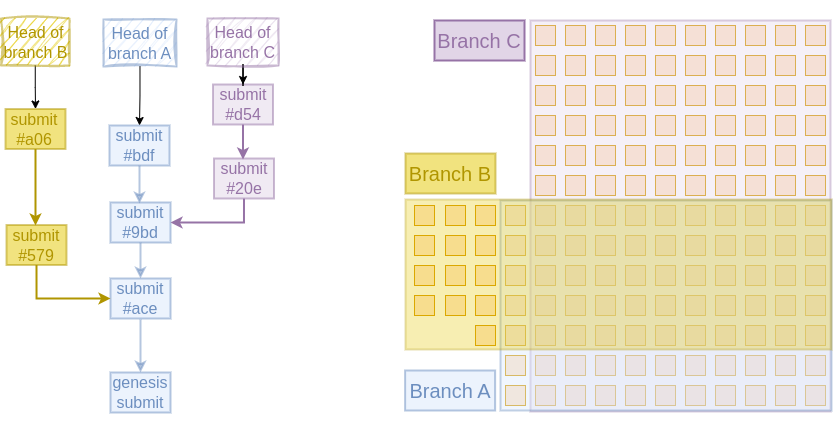
\includegraphics[width=1.0\textwidth]{img/BranchBucketRelationV2.png}
\end{center}
 \caption{}
 \label{fig:branchbucketrel}
\end{figure}

\subsubsection{Storage}
\label{ssc:storage}

% i
The data is stored in key-value databases and is content addressed in the sense that the key equals the multihash of the data. Inside the multihash there is information about the storage protocols used. So if one would use, say ipfs, for storage then a certain flag in the multihash would be raised. If also another protocol or system would be used then this would again be seen through the flag in the multihash. To proof that a certain data bucket has been stored, i.e. pinned, that proof is attached to the mutable information of the bucket in the \textit{storageProofs} entry. There are a few more constraints about storage and pinning. It should be encouraged that every data bucket belongs to at least one molecular bucket so that there are no buckets without a context. Thus when a new data bucket is submitted the submission won't be accepted unless it is present in at least one context bucket.

\subsubsection{Branch--Requests}

Every branch has its own staging area, where any type of branch interactions are waiting to be included. This is called the \textit{Branch--Requests} (or BR in short). It is similar to the mempool in ethereum. Everyone who is participating in the branch (See Protocol \ref{ssc:protocol}) and who runs a light client may receive branch interactions from users and broadcast them to the network. Here we refer to a \textit{client} as a piece of software that is yet to be written, which interacts with the network. A \textit{light client} is a client that is not capable of doing branch operations, but is capable of receiving and broadcasting branch--requests. Inclusion of requests into the branch, however, requires more (see Protocol \ref{ssc:protocol}). There are eight channels in the branch--requests (see Figure \ref{fig:mempool}): \textit{submit requests}, \textit{pull requests}, \textit{review commits}, \textit{review submit requests}, \textit{social transactions}, \textit{token transactions}, \textit{storage updates} and \textit{branch creation broadcast}. The requests inside the BR are not permanently stored. Requests are kept for as long as any of the branch contributors keeps track of them. That is where the similarity to the mempool stems from.

Every channel in the Branch Requests has a certain capacity. In particular this aims to prevent that one channel clutters the entire pool of requests, which might happen if the capacity was channel-independent. All requests or broadcasts are serialized. 
Submit requests contain a serialization of the data buckets that are requested to be added to the branch. Pull requests are simply pings from other branches that seek reviewers. Only by means of a pull request are contributors from the target branch allowed to make modifications to the requesting branch (see Proof of Revie \ref{ssc:consensus}).


\remark{One can submit interaction data to any branch that holds it. Once a branch processes it, }



\begin{figure}[h!]
  \begin{center}
    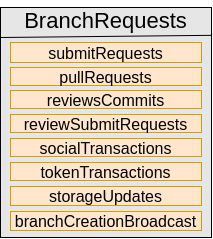
\includegraphics[width=0.25\textwidth]{img/MempoolV3.png}
\end{center}
 \caption{}
 \label{fig:mempool}
\end{figure}

\subsection{Contributors and Contributions}
\subsubsection{Contributors}
\label{ssc:contributors}

Every branch has \textit{contributors}, or rather contributors have branches. A contributor is an account that can prove to have contributed to a given branch. There are four types of contributors for any given branch: \textit{content contributors}, \textit{review contributors}, \textit{token contributors} and \textit{storage contributors}. A content contributor can prove to have submitted to the branch. A review contributor is someone who can prove to have pushed reviews to the branch (see Subsection \ref{ssc:por} for information on proof of review). A token contributor is someone who can prove to have deposited funds into the branch. A storage contributor is someone who can prove to store data of that branch. Being a contributor means that you have to prove your contribution for the submits from the root submit of the branch till the current stable head.
How does the set of contributors change during a merge? What is the relation betwen the contributors of two branches before the marege and after? When the belt branch merged into the core following a pull request, then the new set of contributors is simply the union of the two branches (see Subsection \ref{ssc:branch} for the terms core and belt). That holds for all contributor types. When there is no pull request preceding the merge the contributors of this branch are unaltered.
The main idea behind the concept of contributors is the mutability, governance and autonomy of branches. Branches can only be modified by their contributors. This attempts to preempt attacks on branches.

% 
% Every branch has a history of submits and is \textit{rooted} in some parent branch or is itself a \textit{seedling} (See Subsection \ref{ssc:branch} regarding roots and seedlings). In either cases there is a set of contributors to every branch between its root and the current head. Any actor, human or AI, who is a creator of content in any of the branch's submits counts as a contributor (See Subsection \ref{ssc:contributor}). 

% 
% \subsection{Protocol}
% \label{ssc:protocol}
% 
% 
% The protocol level deals with all those aspects that mutate the data.
% 
% 
% You can only make changes to the branch that you are contributing to. 



\subsubsection{Contributions}
\label{ssc:contributions}


\subsubsection{Proof of Contribution}
\label{ssc:proofofcontributions}


\subsection{Local Consensus}
\label{ssc:localconsensus}

Who decides which content will be added to a branch? In lakat there is no global notion of what counts as science and what does not. There is only a local notion, the detailment of which is the subject of this section. A global consensus mechanism seems to be a good fit for a ledger that keeps track of values that are or ought to be globally agreed upon, i.e. for values that exist qua their global agreement. In contrast to money transactions, the global scope seems ill-fitted for the publication of research content. In our view this requires a local form of consensus. In the context of Lakat, the scope of the locality is at the branch-level. 

What does a branch-level scope mean? This means that the scope is constrained to the \textit{contributors} of a branch. Every branch has a history of submits and is \textit{rooted} in some parent branch or is itself a \textit{seedling} (See Subsection \ref{ssc:branch} regarding roots and seedlings). In either cases there is a set of contributors to every branch between its root and the current head. Any actor, human or AI, who can prove the contribution of content in any of the branch's submits counts as a contributor (See Subsection \ref{ssc:contributor}). 

Branch contributors form the basis of the consensus mechanism. We entrench this deep into the protocol by allowing only branch contributors to make changes to the branch that they are contributing to. This design choice also keeps potential attackers or crackpots from pushing unwanted content to a branch. Lakat does not make statements about what counts as science and what not. What counts as a legitimate scientific contribution purely emerges through the local consensus. One contribution that is viewed as being unfounded or unscientific for one branch might be viewed the opposite on another branch. In some sense this reflects a Feyerabendian approach \cite{}. It gives space for pluralism and allows for the organic selection of branches with possibly differing demarcation criteria. There is, however a positive momentum expected to emerge towards methodic agreements at least across branches that are close to each other. Branches that are close have branched off recently and possibly disagree more on technical grounds than on methodic grounds or they are simply feature branches that are to be merged back in. There is an overall incentive to merge branches, derived from the persistence of the data and the value of the token (see Subsection \ref{ssc:incentive} for possible incentive structures). 

The local consensus paradigm is governing amendments to branches, both to twigs and to proper branches. Sprouts on the other hand are just auxiliary objects that cannot be modified directly and are thus not amenable to a consensus mechanism. The consensus paradigm for twigs simply states that any branch contributor can push submits to the twig whereas merging into a twig requires a certain fraction of contributors to agree (See Subsection \ref{ssc:twigs} for twigs and Subsection \ref{ssc:twiglocalconsensus} for consensus on twigs). For proper branches the local consensus takes on a different form. It is divided into proof of review (See Subsection \ref{ssc:por}), broadcasting and lignification (See Subsection \ref{ssc:lignification}).

\subsubsection{Feature Branches}\label{ssc:twiglocalconsensus}

Twigs are meant to be used for rather quick iteration. They behave like feature branches. Here is an example where twigs are expected to be used: If a contributor, human or AI, would like to add content to a target branch, say an article or some modifications or both, it creates a feature branch rooted in the target branch which subsequently goes through the proof-of-review consensus mechanism (see Subsection \ref{ssc:por}). Typically the number of content contributors on a twig will be low. Maybe a single author or a small group of authors, as it is the case for article publications. In order to not compromise the momentum and the quick iteration both content contributors and review contributors (if there are any) can push to the branch directly. Merges can also be pushed, but require a fraction of approvals of the content contributors. The fraction is determined in the config of the twig. 

\subsubsection{Proof of Review (PoR)}
\label{ssc:por}

Before a branch can be merged into a proper branch it needs to undergo a review. Table \ref{tab:reviewProcess} summarizes the steps.
% % We describe this process keeping to the notation of \textit{belt} as the branch that seeks to be merged and \textit{core} as the target of the merge (see Subsection \ref{ssc:branch} for the terms core and belt).
To start the review process an \textit{issuing branch} creates a pull request from a \textit{requesting branch} to a \textit{target branch}. The pull request is a submit with two properties: First it contains a newly created context data bucket, called the \textit{review container}, that will hold all the forthcoming information of the review. The submit may of course contain other buckets besides that. Second, it leaves a trace of the information about the pull request in the pullRequests entry of the \textit{submitTrace}, namely pointers to the review container, to the target branch and the requesting branch. In most cases the review happens on a twig, which acts as a feature branch. There the issuing branch and the requesting branch are identical, because the twig requests for itself to be pulled into the target branch. However, the requesting branch may also act as a proxy requester. This is the case when a proper branch rather than a twig seeks to be merged into a target branch. Since this intention itself must pass through the consensus rule of that proper branch, one would have to create a twig and include therein the proxy pull request. Once that twig is successfully merged into the actual requesting branch by passing the consensus, the review process can begin on that proper branch for it be mergeable into the target branch. We call a pull request \textit{mature} once it is included in the requesting branch. In the most common scenario where the issuing and requesting branch coincide maturity is immediate. 
% In the ensuing merging process the requesting branch becomes the belt and the target branch becomes the core.}
Once a pull request becomes mature a message will be send to the target branch  where its contributors are invited to review the requesting branch. The message is simply a reference to the pull request sent to the pullRequests channel of the target's \textit{branchRequests} (see Subsection \ref{ssc:mempool} for branch requests).
Any content contributor of the target branch who is not also contributing to the requesting branch can then become a \textit{review contributor} of the requesting branch. They must first publish a review commitment on the requesting branch. This makes them official contributors to that branch. It also helps to gauge general reviewers engangement prior to the actual review. This is helpful both for those who seek to merge and those who seek to review. It also increases accountability of the committing reviewer. Failing to supply a review after a commitment could be penalized via the social engagement (see Subsection \ref{ssc:socialrefs}).  
Committers publish their commitment in the reviewsTrace of the submitTrace. They cannot submit reviews without a prior commitment. Also, the identity of the reviewer is not public in the sense that the commitment solely contains a zero-knowledge proof that the reviewer is a contributer to the target branch (see Subsection \ref{ssc:proofofcontributions}).
Of course the reviewer may decide to reveal their identity and this may or may not be in line with the configuration of the target branch.

Reviewers then push review submits to the requesting branch. The submits just contain a proof of contributorship in the target branch. A review submit consists of the following: A bucket with a review, called a \textit{review item}. This bucket should reference all the data buckets that it has reviewed. In the respective interaction data (see Subsection \ref{ssc:branch}) of all those reviewed buckets a reference to the review item is stored within the reviews entry. Finally the review item gets referenced in the review container of the pull request. Updating the review bucket, as with any bucket update, consists of creating a new review bucket that points to the old one through the parent entry\footnote{In future versions of Lakat we wish to move to updates via deltas.}. The branchConfig of the target branch specifies the pre-requisites for a merge. This consists of the minimum number of reviewers, a rule for acceptance and a minimum number of review rounds, which could be one by default. The rule of acceptance could be preset aswell. For instance one could reject requests when a certain fraction of reviewers reject and accept when there are no rejections and specify some rule for the middle ground. Once all the requirements of the target branch are satisfied the branch is ready to be merged. 

How about merging branches that do not seek to be merged? This can be the case when trying to merge the newest developments from a remote branch. This case is in fact already covered by the respective consensus mechanisms of twigs and proper branches. Merging into twigs requires a fraction of content contributors to agree (see Subsection \ref{ssc:twiglocalconsensus}). Merging into proper branches requires a pull request and subsequent reviews, so it is not possible to just merge other un-reviewed branches in the same way that one merges reviewed twigs or reviewed proper branches. Therefore, one would have to create a twig that merges the remote branch as a feature. It then requests to be merged und the merge undergoes a review. \remark{clarify}



\begin{table}
  \begin{tabular}{|p{0.025\textwidth}|p{0.3\linewidth}|p{0.595\textwidth}|}
  \hline
  \textbf{\#} & \textbf{Step} & \textbf{Description} \\
  \hline\hline
  1 & Create pull request & The issuing branch creates a request for the requesting branch (in most cases identical) to be merged into the target branch. A review container is created. \\
  2 & Maturity of the pull request & The pull request is included in the requesting branch (in most cases immediate)\\
  3 & Commitment & A content contributor of the target branch publishes a review commitment to the requesting branch. That makes them review contributors of the requesting branch.\\
  4 & Review & The review contributors create review submits that are referenced in the review bucket.\\
  5 & Completion & The number of review cycles and the coverage of the review meets the criteria of the target's branchConfig. The branch may be merged into the target.\\
 \hline
  \end{tabular}

  \caption{Overview of the Proof--of--Review (PoR) process}
 \label{tab:reviewProcess}
\end{table}

\subsubsection{Broadcasting and Lignification}
\label{ssc:lignification}

How are the reviewed pull requests bundled up and sequenced into a single proper branch? Why is the process important? How is the required attention bandwidth for this proess kept to a minimum? In order to explain the Lakat answer to this question we first contrast it to the case of blockchains: There transactions are bundled into blocks. They are then broadcasted across the network of nodes. When different blocks with the same parent are broadcasted, there will be conflicting versions of the blockchain state, which for a single source of truth is undesirable. In ethererum prior to the transition from the proof-of-work to the proof-of-stake these alternative versions were called ommers and were mostly the result of latency in the broadcasting, but of course also attacks or client-software issues. To make sure that a transaction has irrevocably been added into the blockchain one would have to wait for a few block confirmations. 

In Lakat we solve the issue through a process that we call \textit{lignification}. The idea is that amongst the potentially plentiful and conflicting versions of the new branch state eventually a new head will be chosen. This head is then called the stable head. The versions are stored as short-lived branches, called sprouts. The \textit{sprouts} entry of the branch points to them. Why is the process of choosing a successor to the stable head important? Here is an explanation: The branch is an object that is kept alive by an ecosystem of contributors. It could get hijacked by a group of bad actors who became branch contributors through a mal-reviewed pull-request. In principle, if this happened, the contributors that disagreed with this malicious onboarding could bail out by creating a new branch. However, this new branch would have to grow the reputation of its contributors anew, seek new storage providers, have a new branch token and would generally have to start from scratch. It might not even be an attack, but a disagreement in the community that leads to a branching.
Even though the process of finding a new stable head constitutes an important security measure for the branch, it should not create an overload of attention demanded from the target branch contributors. In most cases there will be no action required. But it is precisely those rare cases, where such a security measure becomes valuable. So one of the requirements for this process is that the branch production continues unambiguously when there is no interference from the community of contributors. In the following we introduce the process of broadcasting and lignification in more detail.

\paragraph{Broadcasting.}

Henceforth we refer to our proper branch as \textit{core}. Every proposed new merge submit could either become the stable head of core or become the first submit of a new (disagreeing) branch that is rooted in core. We refer to any of those new branches collectively as the \textit{peri} branch. Merge submits carry in themselves the possibility of becoming the head of a new branch. Therefore we decided to "wrap" them into short-lived proto-branches, namely sprouts, whose respective heads are the merge submits. The process of broadcasting is as follows. A content contributor of core, let's call her Alice, creates a merge submit, which is a special kind of submit (see Subsection \ref{ssc:submit} \remark{ToDo}). This submit is then wrapped into a sprout, which means that the head of the sprout is set to be the merge submit and the content contributors are set to be the union of Alice and all the contributors of the pull-requesting branch. Let's call this sprout \textit{S}. The branch information of the sprout becomes relevant if it eventually turns into a proper branch, a process which is discussed in the lignification part of this Subsection. The parent of the merge submit is the head of a branch \textit{B}, that is either the core or any of the sprouts upstream of the core\footnote{The sprouts entry of a proper branch keeps track of all the upstream sprouts, but depending on the last branch update may also contain outdated sprouts. In order to retrieve all upstream sprouts one may "walk" upstream using the sproutSelection entry, which only contains the immediate offspring sprouts of a given branch.}. Alice chooses \textit{B}, so she decides where to root the new sprout. If she decides to point to a branch that is already pointed at, there will be a conflict. The new sprout \textit{S} -- or rather its branchId -- is then added to the sproutSelection entries of \textit{B} and the sprouts entry of the core (which might coincide with \textit{B}). The new state of core is then broadcasted to all contributors of core. Note that the new state of core might have received more updates than just the modification of the sprouts or sproutsSelection entries. There can also be further modifications resulting from the lignification process (see next part). The changes, i.e. creation, of the sprout branch \textit{S} are also broadcasted to its contributors. 

\paragraph{Lignification.}

Once a given submit is the new stable head of core or of peri, it cannot be revoked. We say it is \textit{lignified}. The conversion of a previously flexible object into a rigid amendment of a branch has similarities to the process of lignification in botany. 
The decision about the stable head is not made immediately, but there is a period of time where it can still be revoked and deferred. This time is called \textit{lignification time}. As mentioned above, the objects that we make decisions about are not the merge submits themselves, but the sprouts that contain them. If there is only one sprout available after the lignification time, then the decision is clear, namely that the submit contained in that sprout becomes the new stable head of core and no action is required. However, there may be multiple sprout options. In this case, we propose to have a deterministic rule that singles out one sprout and we suggest the possibility of vetoing the default deterministic choice. This minimizes the need to vote each time multiple options arise, but more importantly it reduces the attack vector for people to bring branch growth to a halt by proposing alternate -- yet still reviewed -- merge submits. Vetoing is possible throughout the lignification time. Any branch contributor may register a veto to any of the vying sprouts and therefore against the default sprout. In case that a veto is registered the sprout in question has a chance to provide the next stable head. \remark{how does that work in practice and where is the veto registered and every proposal of new merge submits can also advance the state of the stable head ...}
Once a veto is registered, the content contributors can bring in their votes on the rivaling sprouts. After a period of time, called the \textit{engagement time}, the winning sprout will provide the new stable head and the other sprouts can turn into peripheral proper branches rooted in core. Like with blockchains, the state of Lakat does not change by itself, but only through transactions (See Subsection \ref{ssc:transaction} for transactions). This means that only when a new submit is broadcasted can the state of a branch be updated. Furthermore, a branch may only be updated if it is the target of a transaction. If the transaction is targeting core, then peripheral branches cannot be updated and vice versa. As a consequence those ousted rivalling sprouts do not turn into their own branches immediately, but only once a transaction targets them. Some of them may never turn into proper branches at all. Apart from the lignification time and the optional engagement time there is a time allowing for latency issues in broadcasting, called the \textit{broadcastingBuffer}. This ensures that the timestamped vetos or votes are broadcasted and thus recorded before the stable head is irrevocably fixed.

Due to the time between successive transactions it is quite possible that the state of the core, in particular its stable head, needs to be updated. Maybe the veto time or the voting time between rivalling sprouts has passed or maybe there are no rivalling sprouts and the stable head simply needs to be advanced. The speudo-code in the Lignification Algorithm \ref{alg:lignification} outlines the iterative procedure that advances the stable head on each new transaction. It is worth noting that also the sprouts entry and the sproutSelection entry of core get updated by pruning and replacement respectively.
An illustration of the lignification process is also shown in Figure \ref{fig:bufferbranches}.

In practice the broadcasting and lignification can be automated by a script so that it requires less cognitive bandwidth. The script would choose a content contributor of core at random and broadcast collect all the pull requests that meet the merge-requirements from core, then create one or more merge submits from them, go through the lignification process and broadcast the result. Only in the case when there are disagreements would a manual interference be required.

\begin{algorithm}[h!]
\caption{Lignification -- Advancing the stable head of the branch}
\begin{algorithmic} 
\STATE checkChildSprouts $\leftarrow$ TRUE
\WHILE{checkChildSprouts}
\STATE sprouts $\leftarrow$ childSproutsOf(targetBranch::stableHead)
\IF{sprouts is empty}
\STATE checkChildSprouts $\leftarrow$ FALSE
\ELSE
\IF {all sprouts are within veto time (plus \textit{broadcastingBuffer})}
\STATE checkChildSprouts $\leftarrow$ FALSE
\ELSE
\IF {the default successor sprout has no vetoing sibling sprouts}
\STATE targetBranch::stableHead $\leftarrow$ defaultSprout::stableHead
\STATE targetBranch::sproutSelection $\leftarrow$ defaultSprout::sproutSelection
\STATE prune all sprouts from targetBranch::sprouts that aren't upstream from targetBranch::stableHead.
% \STATE prune sprout from targetBranch::sprouts and targetBranch::sproutSelection
% \FOREND
\STATE checkChildSprouts $\leftarrow$ TRUE
\ELSE
\STATE /* one ore more siblings have vetoed */
\IF {voting has finished, i.e. engagementTime is over}
\STATE targetBranch::stableHead $\leftarrow$ winningSprout::stableHead
\STATE targetBranch::sproutSelection $\leftarrow$ winningSprout::sproutSelection
\STATE prune all sprouts from targetBranch::sprouts that aren't upstream from targetBranch::stableHead.
\STATE checkChildSprouts $\leftarrow$ TRUE
\ELSE
\STATE checkChildSprouts $\leftarrow$ FALSE
\ENDIF
\ENDIF
\ENDIF
\ENDIF
% \STATE $X \leftarrow 1 / x$
% \STATE $N \leftarrow -n$
% \ELSE
% \STATE $X \leftarrow x$
% \STATE $N \leftarrow n$
% \ENDIF
% \WHILE{$N \neq 0$}
% \IF{$N$ is even}
% \STATE $X \leftarrow X \times X$
% \STATE $N \leftarrow N / 2$
% \ELSE[$N$ is odd]
% \STATE $y \leftarrow y \times X$
% \STATE $N \leftarrow N - 1$
% \ENDIF
\ENDWHILE
% \FOR {$sproutPtr$ in $branch::sprouts$}
% \STATE $sprout \leftarrow $ sproutAt($sproutPtr$) 
% \IF {timestamp($sprout$) $\leq$ timestamp($stableHead$)}
% \STATE del $sproutPtr$ from $branch::sprouts$
% \ENDIF
% \ENDFOR
\RETURN
\end{algorithmic}

\label{alg:lignification}
\end{algorithm}



\begin{figure}[h!]
  \begin{center}
    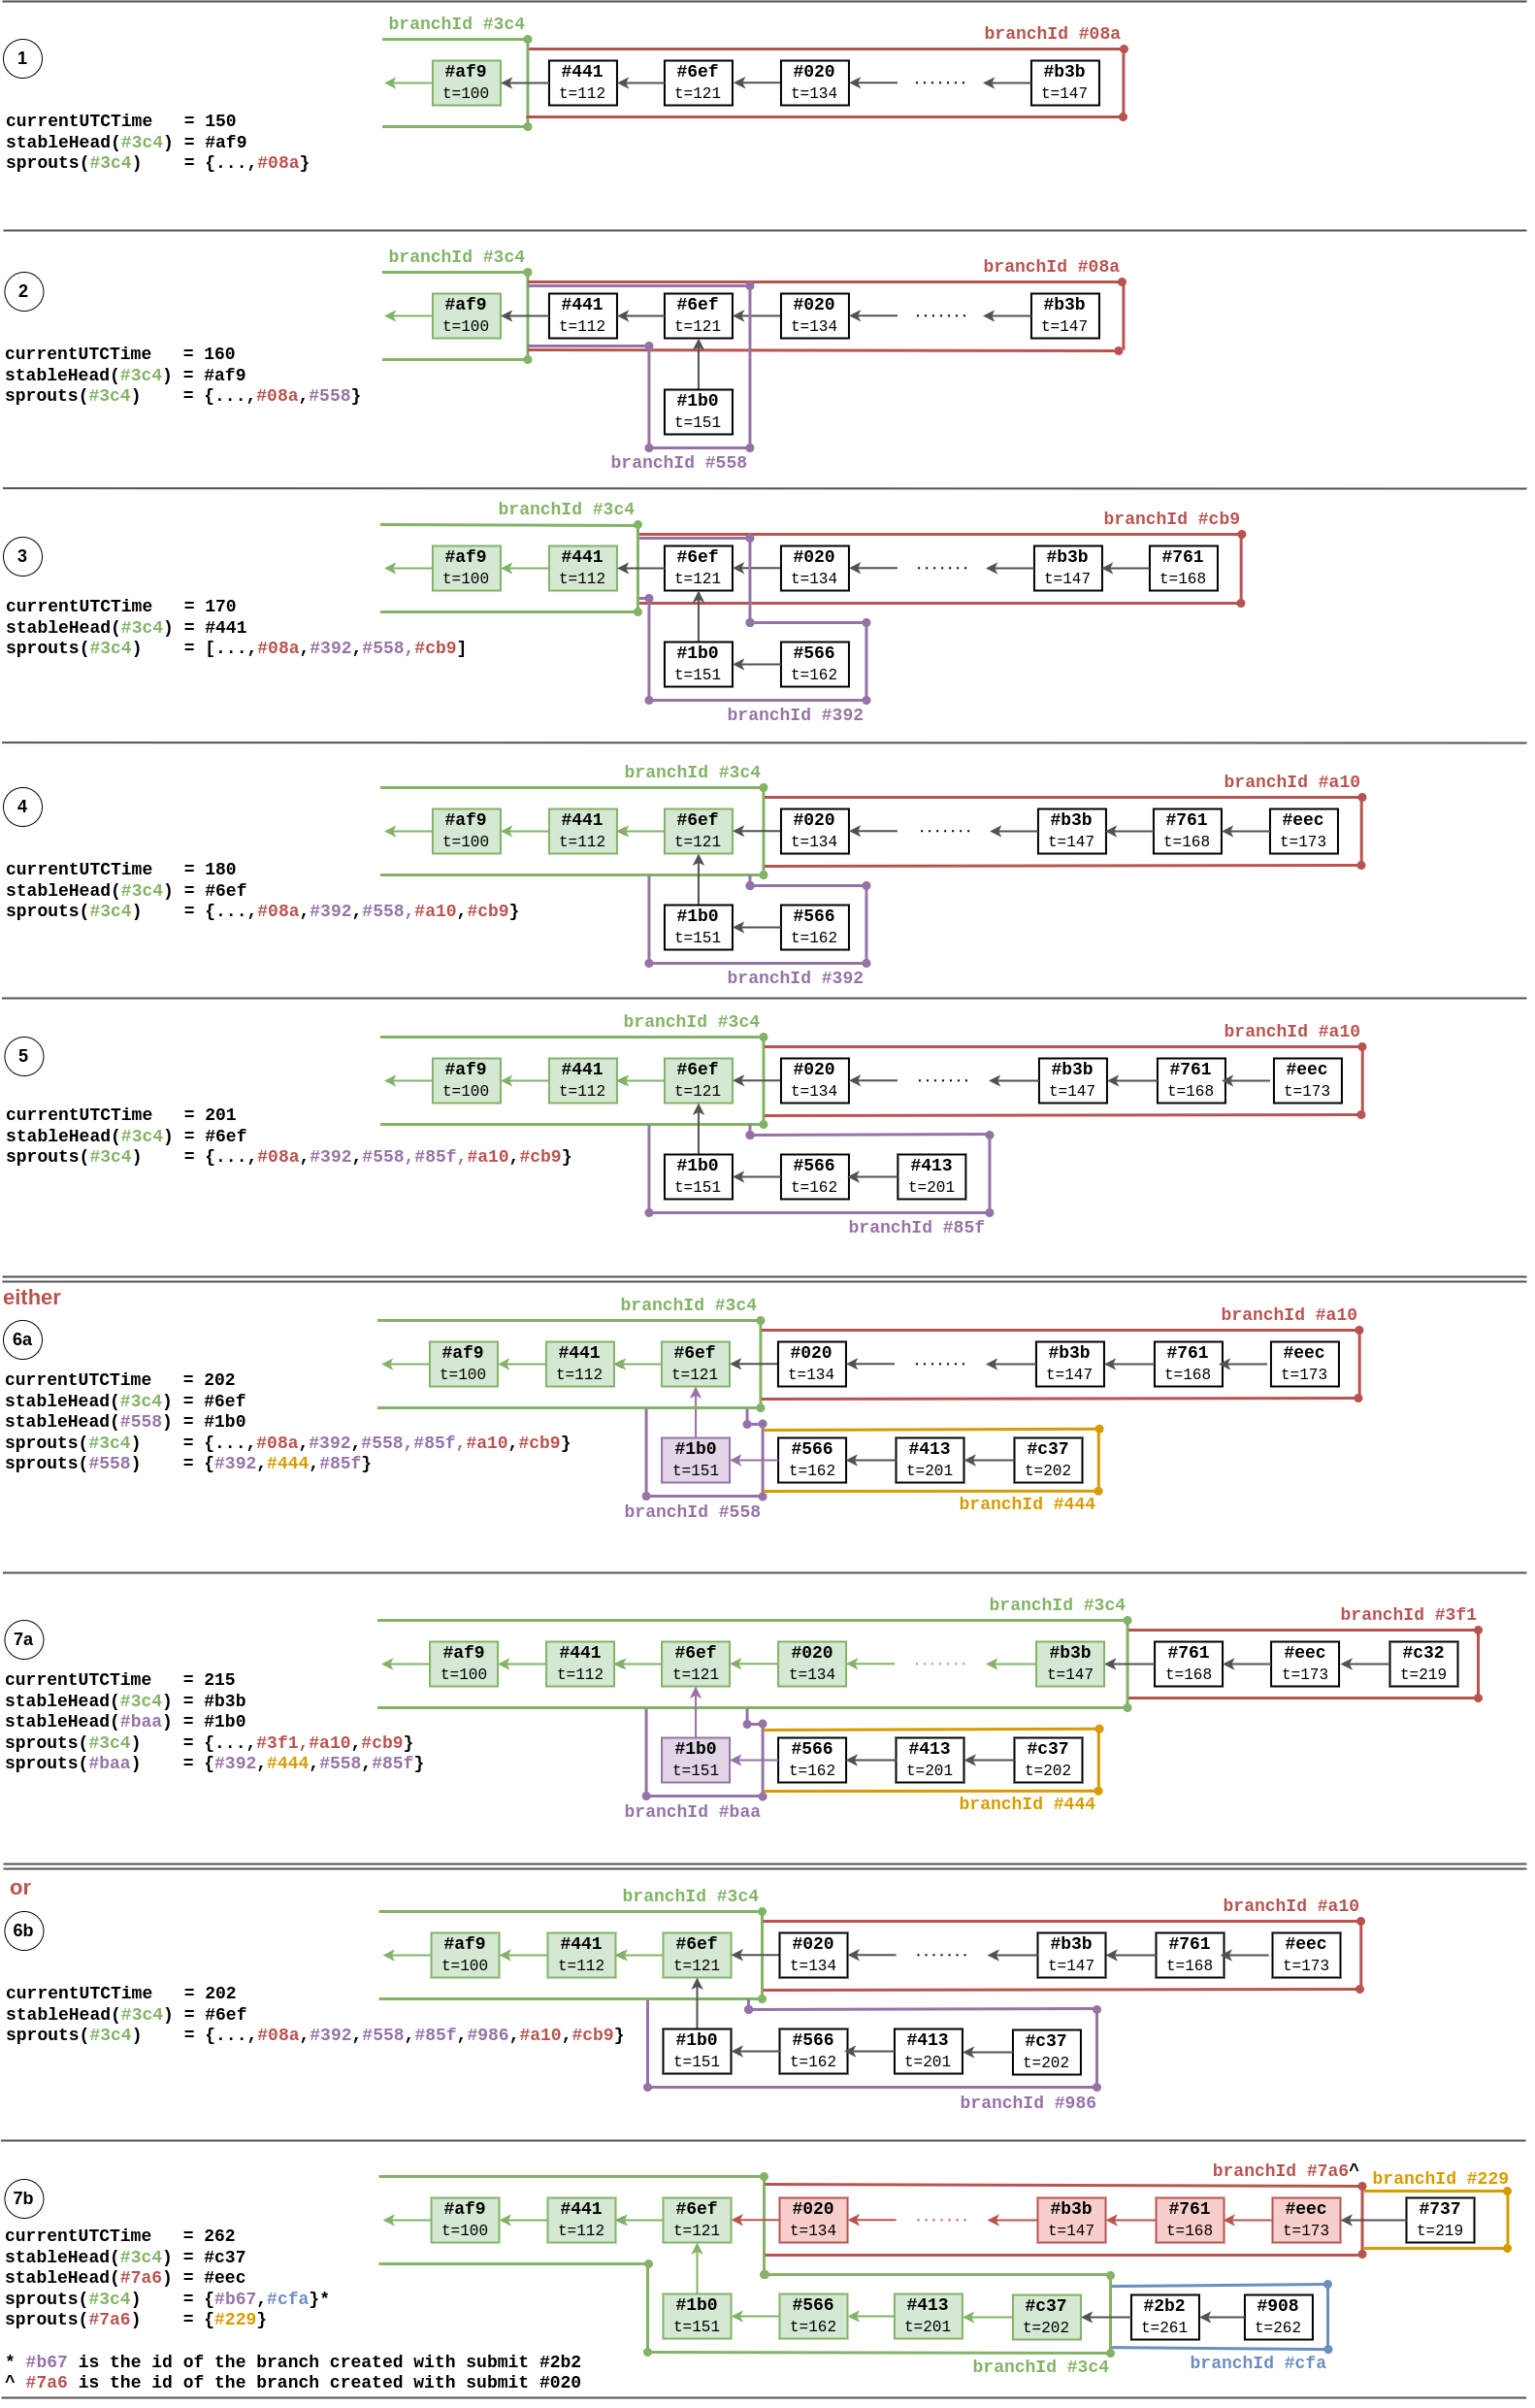
\includegraphics[width=0.79\textwidth]{img/LignificationProcessV5.png}
\end{center}
 \caption{A hypothetical example of a branch lignification for the following example branch parameters: \textit{broadcastingBuffer} $=1$, \textit{lignificationTime} $=50$ and \textit{engagementTime} $=60$. Updates 1 to 5 are within the veto time. There are two optional further paths. Either no veto is given, which is the path from step 6a to 7a, or a veto is given at the last possible time of $t=201$ ($=t$(contestor) + \textit{lignificationTime}) through the submit \textit{\#413} at Step 6b. Here the contestor is the submit \textit{\#1b0}. In this hypothetical scenario the contributors of the stable branch \textit{\#3c4} vote in favor of the contesting submit. The new stable part of the branch is thus decided in Step 7b.}
 \label{fig:bufferbranches}
\end{figure}


% Comparison to the blockchain case



\subsubsection{Branch Config Changes}

% \subsubsection{Branch Type Changes}

\subsubsection{Branch Operations}
\label{ssc:branchops}

The first branch operation is the creation. There are two types of branch creations and three ways they come about. The most basic type of branch creation is a genesis branch without a parentBranch. A branch can either be rooted in another branch or it can be created as a genesis branch with an empty root. \remark{get rid of parentId in branch}


Merge, 

creation, 



Creating a new branch does not require any consensus. One may broadcast it to some other branches, but there is no way for anyone to impede a branch creation. 

password recovery.  ... upon contribution you receive a share


How many contributors should agree for a submit and how many rounds of reviews for a merge. All those are inside the branchConfig.
The presets are themselves buckets. Like whether the amount of agreement for a staged submit to be included in terms of score. 




\section{User Flows}

\section{Attack Vectors}

% \remark{schema of the parent needs to be the same.}



% 
% We use a schema to distinguish the bucket types and  
% 
% We opt against a folder structure, where
% There are no objects that represent folders, such as in git or unix. The limitation that comes with a folder structure is that content can not be part of two or more folders. It requires the hack of soft and hard links to emulate that.



% 
% 
% A submission contains a proof 
% 
% 
% 
% \subsection{Proof of Review -- A local consensus}
% 
% Who decides from whom which contribution should be published? If there was a global consensus about what is a legitimate contribution we would either need one 
% 
% 
% At a high level we propose a permissionless, open and distributed database with a local peer-reviewed concensus layer. Data is submitted as a set of proposed changes rather than in bulk. It may be viewed as a CI/CD solution for publishing and one may conceptionally think of Lakat as a decentralized form of wikipedia with branch structure and peer review. Its primary use case is publishing of research output. We present the core architecture and then dive into the individual choices in more depth. 
% 
% 
% 
% Content is 
% 
% 
% 
% The proposed publishing system is a distributed multibranch version control system. We first provide a high level overview of the elements and then discuss them in more detail, \remark{starting from the requirements that we aim to satisfy.}
% 
% 
% Can only merge when the molecular and atomic content satisfies. a relation. 
% 
% \subsection{Overview of the Elements}
% 
% 
% What is the structure of content? Rather than relying on a folder structure, as is the case in \href{https://git-scm.com/}{git}\cite{torwalds} or \href{https://en.wikipedia.org/wiki/Unix_filesystem}{unix}\cite{unix}, we propose to build the publishing system on content buckets, called \textit{atoms}, and context buckets, called \textit{molecules}. For all practical purposes one may think of atoms as the smallest unit of published content such as captions, paragraphs, formulae, arguments, media files, data sets etc. Small chunks of content allow for better reusability and updateability. Molecules on the other hand can be thought of as content containers such as review articles, book chapters or monographs. They put atomic content into a context. Atoms can be part of multiple molecules, which is not possible in a folder structure.
% 
% How is new content submitted? It is submitted in terms of changes, rather than in standalone bulk. A submitted change is called a \textit{submit}. 
% %Thus a submit is merely difference, rather than a snapshot. This is also reflected in the data storage (see Subsection \ref{ssc:storage}).
% A submit alters and references a previous submit, the \textit{parent submit}. Every submit is comprised of changes to the individual atoms and molecules and has a unique history of submits that includes itself and all of its parent submits. This history is is called a \textit{branch} and uniquely identified by its latest submit. The content of one branch may be included into that of another branch, a directional procedure referred to as a \textit{merge}. Branches may have conflicting content. When attempting to merge one branch into another with conflicting content a \textit{merge conflict} arises that should be \textit{resolved}. The overall structure of submissions will be an arbolescence\footnote{For information about the graph-theoretic term of an arbolescence refer to \remark{TODO}.}, a directed tree called the \textit{submitree}. 
% \remark{Making conflict resolution manifest}
% 
% Likewise, at the level of atoms and molecules, there is a linked data structure. The atoms and molecules are arbolescences, called  \textit{atomic submitrees} and \textit{molecular submitrees} respectively. They tend to be less branched, since not every branching submit alters every single atom or molecule. We add \remark{better formulation} a remark on the design choice of submitrees at the bucket level:
% Once we allow pieces of content to be reuseable and therefore identifiable and addressable, any branching or merging has to keep track of these bucket identities. However, since there is no preferred branch, we consequentially need to branch (whilst preserving the identity) also the altered buckets and only those. 

% What is the data model for this structure? Like with git and many decentralized protocols, we propose to use a data structure that allows for easy and fast resolution of data using content addressing via cryptographic hashes.   
% 
% What is the relation between submits and branches at the level of atoms and molecules?
% One may think of content and context buckets, i.e. atoms and molecules, as 
% 
% Data model .
% 
% Every submit is identified by a submit hash. We explain the calculation of the hash as well as the resolution of content through the hash. To this end we first note that every submit is uniquely determined via the reference to the parent submit \textit{and} a snapshot of its content. The snapshot of a submit's content, which we call a \textit{section}, is a collection of the atomic and molecular snapshots of all the atoms and molecules that make up the content. They include the snapshots of the changes in the current commit, but going back in the branch history also include the snapshots of other atoms or molecules changed in previous submits. O 
% 
% that have been added in the submit history of the branch. They also include those snapshots of the changes in the current submit. In order to cryptographically secure the content against tampering one may calculate a hash from the snapshot. 
% 
% whereby we mean   
% is a snapshot of its content. is uniquely determined by the atomic and molecular snapshots
% 
% The submit hash is calculated as the Merkle root of all the atomic and molecular snapshots that comprise its content. Those are of course the ones that were altered in that particular submit, but moreover also all the other  It can also resolve the   
% 
% How is data stored?
% 
% 
% 
% 
% 
% have just one universal type of container.  
% 
% 
% Contrary to \textit{git} \remark{or the \textit{unix} file system} there is 
% 
% \subsection{Rest}
% 
% 
%  
% 
% This paradigm facilitates a more continuous and organic content evolution compared to article or monograph submission, but at the same time contains those as special cases.
% 
% conflicts become manifest
% 
% It is more akin to the content growth in 
% 
% that encodes the change a is not a standalone article, but in the format of a change. with reference to a branch, that is a unique history of changes.  
% 
% Published data is stored in a distributed hash table and addressed via an IPLD encoded hash linked data structure. 
% 
% \subsection{Data Structure and Data Storage} \label{ssc:datastructure}
% 
% Like other versioned data structures, such as \textit{git} or \textit{ceramic}, we propose to use content identifiers (CIDs) to reference data and to use Merkle DAGs to aggregate CIDs. 
% %The \href{https://ipld.io/docs/data-model/kinds/}{ipld}
% 
% 
% Data is either content bearing or referential data, i.e. data that references or addresses data. 
% 
% Like most distributed systems, we propose that data is stored by  content addresses
% We describe now the proposed data structure and data storage. 
% 
% 
% We propose a system where research content is grown continuously on a sharded database. \textit{local consensus}
% 
% \subsection{The state}
% 
% There are branches and there are 
% 
% \subsection{Submission}
% \label{ssc:Element_submission}
% 
% enemy of science is personal agendas.
% single ... interests as gate keeper
% 
% try to avoid ideas from being gated away...
% 
% A \textit{submit} is similar to a commit in \textit{git}. It contains a pointer to the parent  contains a number of 
% 
% \subsection{Storage}
% 
% \subsection{Consensus}
% The tasks and purpose of editors and reviewers are all subsumed under the local consensus algorithm.
% 

% This system can be implemented simply by having any contributor write their own research blob








% are still using the format of mostly static so-called papers. T

% .... and our scientific output behaves like physical paper in the way it is treated and guarded by publishers.

% igital form by now, they a still physical  guarded by publishers and paywalls.   

% at our to match requirements to 

% has bee  we not matched our needs with the available technology.
% Publicising ideas and insights depends on the publicising technology. 

% Spoken language, for instance, allows people to make their ideas public inside gatherings and only for that duration. A written cuneiform language allows people to make their ideas public even outside of gatherings and for a long duration, but only at the physical scripture location. Ink and papyrus allowed people to spread their ideas beyond that immediate location. The printing press allowed people to disseminate multiple copies of a scripture, thus addressing a larger audience, a process that akin to modern day publishing. Electronic data processing on a single processor allowed for the inexpensive, fast and scalable way of modifying, reusing and storing content. Networked processors allowed for quicker dissemination and distributed storage.

% With the tool of a spoken language people could make their ideas public inside gatherings and for the duration

% The available publicising technologies are bounded by the available technologies.

% So, both the process 

% These two plain statements   which in turn is bounded by the technological means. 



% This dependence regards the process as well as the  

% is related to the publishing technology that enables the publication.  


% \section{Requirements}
% 
% % Imagine two extreme scenarios. 
% 
% In the first scenario, we keep a single book of scientific "truth". Everything that has been found true for ever after should be written into that book in a cumulative and immutable way. Two questions immediately arise: Who writes and what is true? If a single person or entity writes, then where does this entity take its legitimacy from. If more than one person or entity write, then how can they find a consensus and how can a consensus even be guaranteed in the first place? Moreover, if truth was so easily established, they why are scientists that divided with respect to their results and why do seemingly consensual results get overthrown again and again. It will be hard to argue for this scenario as an appropriate system to produce scientific output. Yet, this system is one that is very much in line with a popular conception of science as an linearly growing accumulation of truths. A positive feature -- if any -- is its clear direction of progress. In order to implement such a system, the alleged truths could be written into a single database and the mighty author would be a generally trusted person or entity. Alternatively, if writing was done through a consensus algorithm, one could implement this scenario as a blockchain.
% 
% Let us now consider another scenario on the other end of the spectrum. Results are being published in lots of small, isolated and self-contained blobs without any agreed consensus mechanism  how to bring them in agreement. The question that can be raised, is how discrepancies are resolved and who resolves them. As was the case for the former scenario, this one is also hypothetical and likewise not an appropriate system for publishing scientific output. Yet, one can argue that this system features similar aspects to the one we currently witness, which has different kinds of consensus mechanisms regarding the acceptance of research output, that are nevertheless not always overt. 
% This scenario has several drawbacks. There is no clear path of resolving discrepancies. One major advantage is that pluralism of research outputs is built into this scenario.  
% 
% A publishing system should live somewhere in the middle ground from these two scenarios. The system should allow content to be grown dynamically, discrepancies to be made visible, consensus mechanisms to be overt and pluralism to be manifest. %% something about storage.
% 
% \section{Distributed Publishing System}
% Everyone may connect to the network and send a \textit{submit} into the network.
% 
% \subsection{Data Structure}
% 
% The smallest unit is a \textit{blob}\footnote{This terminology is borrowed from \textit{git}.}. There are two types of blobs, those that carry content and those that carry context. We call the content blobs \textit{atoms} and the context blobs \textit{molecules}. A typical content blob would be 
% 
% 
% 
% \section{Rest}
% 
% Each technology 
% 
% 
% We are free to choose our form of 
% 
% Progress in or of science has ever since been a field of inquiry.
% Mapping the human undertaking of acrueing knowledge 
% 
% There have been many metaphors, that have been worked out to greater or lesser extend in an effort to map this undertaking. 
% 
% "Wissenschaft", "Fortschritt", "advance" (directional).f
% 
% These metaphores range \footnote{We don't intend to imply a one-dimensionality.} form cumulative processes to growing and waning socio-epistemic ecosystems. Even though it is not fair to speak of metaphores of one and the same thing here. The cumulative approach to science is different in terms of ontology and outlook from the Lakatosian for instance. 
% 
% The interesting thing is that there is such a strong mismatch of the perceived metaphor from the operationalized one. From conversation with people and reading of articles it becomes apparent that more or less science is progressing cumulatively. Yes, people know that there are various schools, that see things differently, but somehow there is this one thread of science, where the loose ends are tied together. This is a common view. On the other hand we have an actualization of our research in research paper publications, reviews and monographs. So more like a set of beats loosely attached to each other.
% It is this divergence that we would like to address.


% 
% This process is mapped to our publishing methods.
% 
% Given our current technological means it would be fair to raise the point whether we can map 
% 
% 
% How could we use our current technological status to build a new science? A thought experiment.
% 
% 
% % \section{Data Architectures of other systems \red{better word}
% \section{Data Architectures \remark{(of other knowledge systems)}}
% 
% \subsection{git}
% At its heart git's data model is a Merkle tree. 
% git is a merkle tree. It 
% 
% % \href{https://initialcommit.com/blog/git-bitcoin-merkle-tree}{blaaaa}
% 
% \subsection{ethereum}
% 
% \subsection{wikipedia}
% 
% \subsection{traditional publishing}
% 
% % \subsection{}
% 
% 
% 
% \section{A survey}
% 
% The way that science is done depends on the incentive / reward system as well as the output system. Although it is surely not right to disentangle them, we just do it nevertheless and cut away a little bit of the complexity involved. We want to survey a few extreme cases. We want to give a very high level, topological analysis, rather than a technical low level analysis here. 
% 
% Why not be brave and turn this into practice. 
% 
% Perpetuation:
% \begin{itemize}
%     \item Verbal communication
%     \item One single book with millions and millions of chapters
%     \item Millions and millions of papers
% \end{itemize}
% 
% Incentives:
% \begin{itemize}
%     \item Names associated to contribution
%     \item Citations 
%     \item The greater good of humanity
%     \item social prestige ...
% \end{itemize}
% 
% % \subsection{verbal communication}
% \section{Literature}
% 
% In \cite{tenorio2019towards} ... they propose that the reward system comes from cryptocurrency. However any reward solution should come from within the framework, otherwise all the advantage of decentralization is lost.(p.4637) ... Who is the editor, who will invite, who is invited.
% 
% "In the event of a
% reviewer sending a review when the time has expired,
% a penalty is applied to the reviewer’s reputation in the
% reputation system." This is a very hardcoded and not emergent border. 
% 
% Blockchain is for absolute values a wonderful technology. The problem that blockchain solved is the 
% 
% \section{A commit network}
% 
% No single truth build in!
% 
% One single ledger. Many branches. Different kind of activities. 
% Contributions are commits. 
% 
% Advantange: If one wants to rely on another result one would have to find the diff.
% 
% It should allow for the plurality. Where would you want to draw the line between crack-pottery and science. It's hard. Well don't. No one can and no one should. There will be branches that are more main stream and those that are less. They should not be censored. 
% 
% Who should keep the entirety of the wisdom? There is really only one answer here: Everyone who participates. Knowledge is too precious to have it on a server or to have it in the hands of a few. 


% There should be somethin like a local consensus. A consensus that is directed at a branch. So every branch is like a block chain. Consensus on that branch is like a pull request. Then there can of course also be merges and forks. 
% 
% As a new-comer you can either fork off somewhere or you contribute somewhere. 
% 
% Every participant of one branch has only their branch as a blockchain. 
% 
% Question: What about tempering. How easy is it to troll the network? Any troll should be able to open a new branch, why not (but somehow you wouldnt want that to go into a storage that is shared by everyone, otherwise it would be an attack vector for DoS). 
% 
% Lets make the terminological distinction between stem (like fork) and branch. A branch can be merged into a stem by pull request and consensus, but a stem cannot be merged simply into another stem without the consensus of their community leaders. 
% 
% One can build a new stem by cherry picking other stems. Every stem keeps its data. That prevents trolls from spamming the entire network.
% 
% Some archival nodes can choose to select which stems to display. 
% A user can then choose between one of the versions and also get the diff! 
% 
% Any node can always be queried of course, but there is a threat that you will be lost in oblivion. But actually this threat is what we are anyway faced with. Something doesnt get published. It will be lost in oblivion!
% 
% ANd this system would lend itself ideally for all sorts of reputation schemes. Such as anonymizing the network or commits will emerge as something reputable. 
% 
% Pseudocode:
% 
% 
% \section{Protocol}
% 
% \subsection{Objects}
% There are three types of objects: atoms, worldlines and contexts. 
% Atoms can be thought of as the smallest unit of a submission, e.g. paragraphs, data items or media files. A worldline is a history of atoms that are connected through deltified updates. They can be thought of as the various versions of an atom. A context provides a higher-level semantic environment for the worldlines. One may think of a context as a paper, a wikipedia entry or a collection of data. All atoms have the same structure and all contexts have the same structure. There is no difference between an atom that holds an image file or an atom that holds a comment.  
% 
% Atoms contain metadata, data and links. Let $A$ be an atom. Its metadata is made up of an identifier $\textrm{id}_A$, a timestamp $\tau_A$ and a pointer to a data decoder ${}^{\star}\!dec$. Its data is bytes-encoded. The link is an ordered list of atom identifiers.
% 
% The context contains metadata and and atoms. There must always be at least one atom, that accounts for the organisation or the arrangement of the context. We call it $O_{\mathcal X}$. Then there is an arbitrary amount of atoms $A_{\mathcal X}, B_{\mathcal X}, \dots , Z_{\mathcal X}$
% 
% \subsection{Opcodes}
% 
% \begin{center}
% \begin{tabular}{ | m{19em} | m{6em}| m{6em} | } 
%   \hline
%   \textbf{Opcode} & \textbf{args} & \textbf{reference} \\
% \hline
%   \hline
%   CREATE\_ATOM & cell2 & \ref{sssc:CREATE_ATOM} \\ 
%   \hline
%   UPDATE\_ATOM & cell2 & cell3 \\ 
%   \hline
%   \hline
%   CREATE\_CONTEXT & cell2 & cell3 \\ 
%   \hline
%   ADD\_CONTEXT\_TO\_ATOM & cell5 & cell6 \\ 
%   \hline
% REMOVE\_CONTEXT\_FROM\_ATOM & cell8 & cell9 \\ 
%   \hline
%   \hline
% \end{tabular}
% \end{center}
% 
% 
% \subsubsection{CREATE\_ATOM}
% \label{sssc:CREATE_ATOM}
% A new atomic item is created. As arguments it takes the pointer to the context ${}^\star\!ctx$.

\bibliography{lib/aDistributedPublicationSystem}
\bibliographystyle{plain}
\end{document}
